% Build from this directory: lualatex -interaction=nonstopmode -halt-on-error mtg_1130.tex
% The figures are derived from the sign-corrected 30--90 s analysis, f <= 0.5 Hz.
\documentclass[a4paper,10pt]{ltjsarticle}
\usepackage[margin=18mm,top=16mm,bottom=18mm]{geometry}
\usepackage[haranoaji]{luatexja-preset}
\usepackage{amsmath,amssymb,bm,graphicx,booktabs,array}
\usepackage[hidelinks]{hyperref}
\usepackage{fancyhdr}
\pagestyle{fancy}\fancyhf{}
\fancyfoot[L]{\footnotesize 2026年11月30日 チームMTG}
\fancyfoot[R]{\footnotesize\thepage}
\renewcommand{\headrulewidth}{0pt}\renewcommand{\footrulewidth}{0pt}
\setlength{\parindent}{0pt}\setlength{\parskip}{4pt}
\setlength{\abovedisplayskip}{6pt}\setlength{\belowdisplayskip}{6pt}
\newcommand{\wrap}{\operatorname{wrap}_{[-180^\circ,180^\circ)}}
\newcommand{\ii}{\mathrm{i}}
\newcommand{\COM}{\mathrm{COM}}
\newcommand{\head}{\mathrm{head}}
\newcommand{\sect}[1]{\vspace{4pt}\textbf{\large #1}\par}
\begin{document}
{\LARGE\bfseries 頭部とCOMの視覚刺激応答}\par
2026年11月30日 チームMTG\quad /\quad 11月24日計測の予備解析\par
{\small 作成日 2026年11月27日}

\sect{結果の要点}
単一リンク近似を用いる解析範囲として\textbf{0.5 Hz以下}に限定し、
最初の1周期を慣らしとして除いた\textbf{30--90秒の3周期}を主解析とした。
符号修正後、大坪の0.20--0.45 Hzでは頭部とCOMが同位相付近だった。
一定の伝達遅れは確定できず、旧処理による「約180度差」は採用しない。

対象は瀬口・大坪・たかとの等速度マルチサイン各1試行。
評価する励起周波数は
\(f=\{0.05,\,0.10,\,0.20,\,0.30,\,0.45\}\,\mathrm{Hz}\) の5点。
0.50 Hzの励起点はない。0.5 Hz以下で単一リンク近似が成立することを、
今回の解析だけで証明したものではない。

\begin{center}
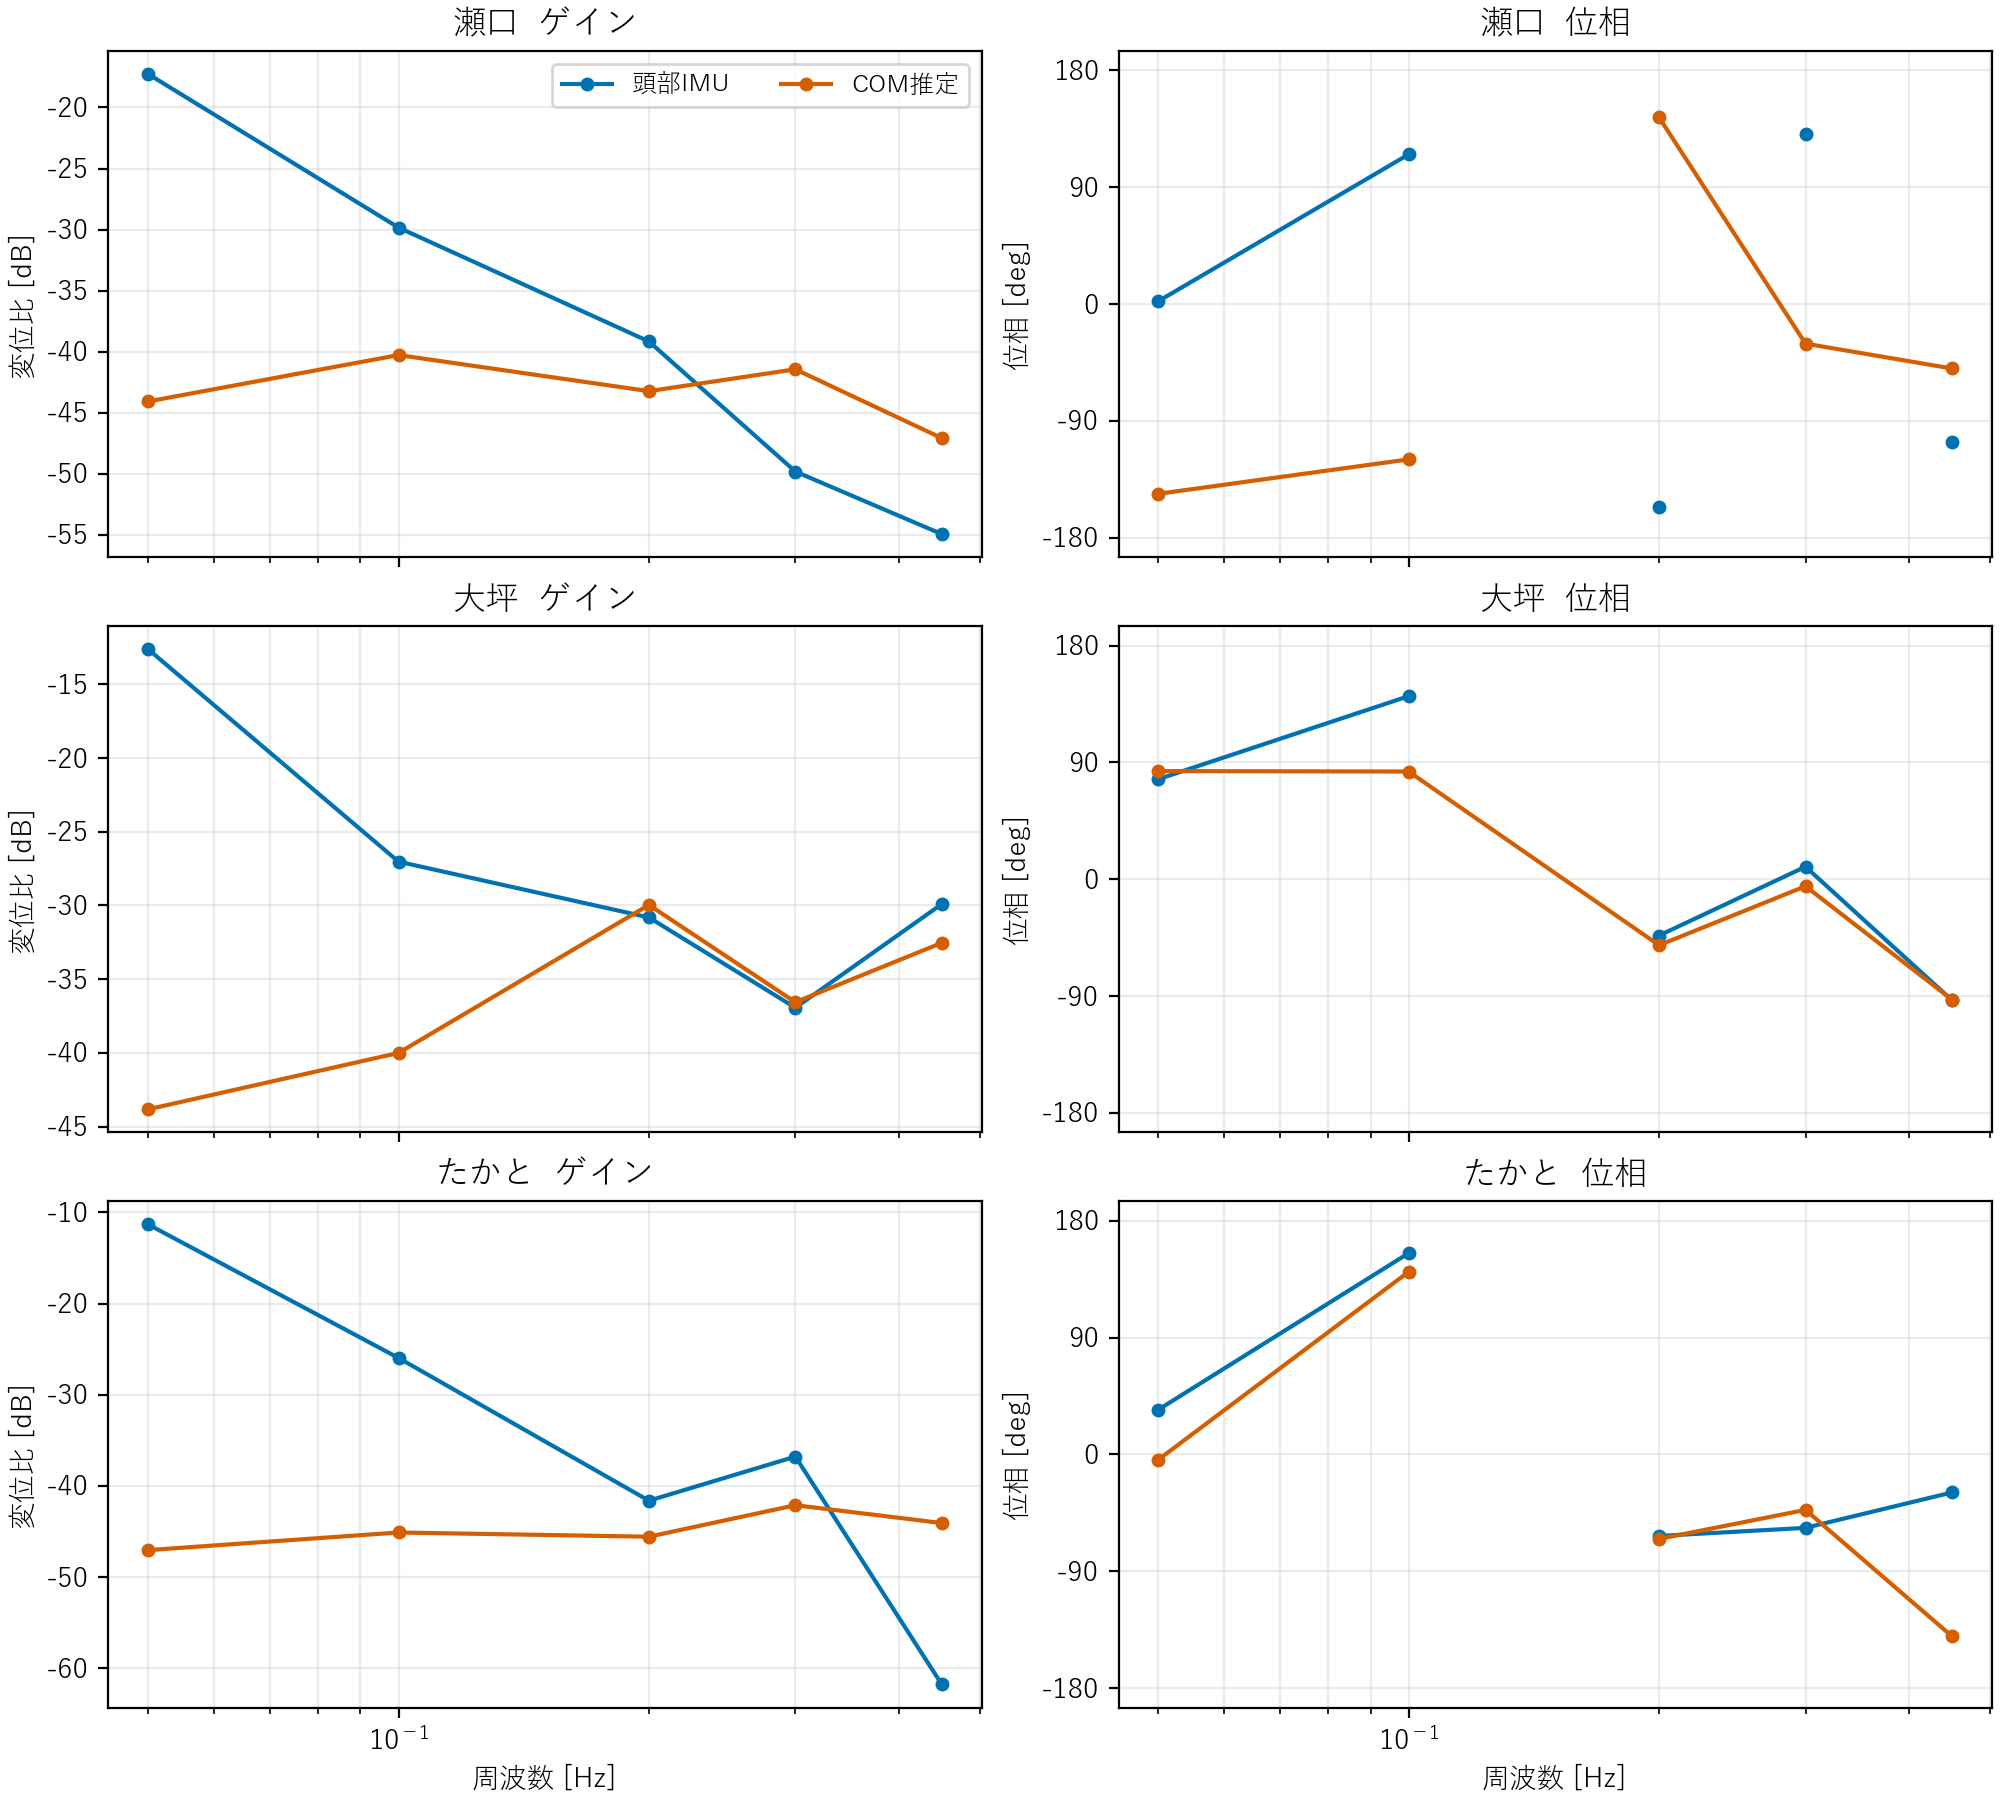
\includegraphics[width=0.96\linewidth,height=160mm,keepaspectratio]{figures/gain_phase_displacement.png}
\end{center}
\vspace{-4pt}
{\small\textbf{図1}\quad 刺激変位を入力、頭部変位またはCOM推定位置を出力とした周波数応答。
青は頭部、橙はCOM。点は励起周波数、線は点の接続。
頭部変位は重力補正済み加速度の周波数成分から算出した。
位相の折り返し境界では接続線を切っている。}

\newpage
{\LARGE\bfseries 解析に用いた式}\par
単位は m、s、N、N\,m。入力と出力の変位・速度・加速度の9組を計算し、
概要図では変位入力・変位出力を示す。

\sect{1 COM位置の推定}
メーカー前後軸変換と接触面への原点補正を、
\begin{equation}
 R_x=F_y,\qquad N_y=M_x-h_0F_y,\qquad h_0=0.0123\ \mathrm{m}
\end{equation}
とし、既存の単一リンク推定式を用いた。
\begin{equation}
 x_{\COM}=\frac{N_y-cR_x}{m_b g},\qquad
 c=\frac{J_b}{m_b l_b}+L_f+l_b,\qquad g=9.80665\ \mathrm{m/s^2}.
\end{equation}
身体係数は以前の解析と同じ男性係数を使用した。
\begin{equation}
 m_b=0.978M,\quad J_b=0.0473MH^2,\quad
 l_b=0.513H,\quad L_f=0.039H.
\end{equation}
\(M\)は静止鉛直荷重からの推定質量、\(H\)は身長、\(m_b\)は足部を除く身体質量、
\(J_b\)は身体慣性モーメント、\(l_b\)は足関節から身体COMまでの距離、\(L_f\)は足関節高さ。
右踵落とし確認時と同じ配置に合わせ、旧処理の\(N_y=-M_x\)を修正した。
水平力の実機校正と個別身体係数の検証は残る。

\sect{2 頭部加速度の重力補正}
\begin{equation}
 a_{\head}(t)=\bm e_{\mathrm{AP}}^{\mathsf T}
 \left[R(t)\bm a_{\mathrm{sensor}}(t)-g\bm e_{\mathrm{up}}\right].
\end{equation}
校正済みの加速度とジャイロから姿勢\(R(t)\)を推定する。
刺激前2秒を初期基準とし、加速度で重力方向へ補正する時定数は30秒。
\(\bm e_{\mathrm{AP}}\)は初期センサ\(+Z\)を水平面に投影した前方向。
並進と重力の分離は暫定的である。

\sect{3 周波数成分の同時最小二乗推定}
\begin{equation}
 y(t)=b_0+b_1(t-\bar t)
 +\sum_{k=1}^{10}\left[a_k\cos(2\pi f_kt)+b_k\sin(2\pi f_kt)\right]+\varepsilon(t).
\end{equation}
定数・直線トレンドと全10励起周波数を同時に推定して、高周波成分も分離する。
\textbf{図示・位相差・遅れの評価には0.5 Hz以下の5点だけを使用する。}
\begin{equation}
 Y(f_k)=a_k-\ii b_k,\qquad s=\ii2\pi f,\qquad V=sX,\quad A=s^2X.
\end{equation}
頭部は加速度から\(X_{\head}=A_{\head}/s^2\)、\(V_{\head}=A_{\head}/s\)を求める。
COMは推定位置から速度・加速度へ変換する。
このCOM加速度は位置の2階微分であり、\(F_y/M\)とは区別する。

\sect{4 ゲインと位相}
\begin{align}
 H(f)&=\frac{Y(f)}{U(f)},&
 G_{\mathrm{dB}}(f)&=20\log_{10}|H(f)|,& \phi(f)&=\arg H(f),\\
 \Delta\phi(f)&=\wrap\!\left[\phi_{\COM}(f)-\phi_{\head}(f)\right].&&&
\end{align}
\(U,Y\)は入力・出力の複素振幅。同じ入力・出力次数で比較すると、
頭部とCOMの位相差は9組で共通になる。

\newpage
{\LARGE\bfseries 位相差と次に確かめたいこと}\par
主解析は30--90秒の3周期、0.5 Hz以下の5点。
位相差はCOMから頭部を引いた値で、正は進み、負は遅れを表す主値。
大きな位相差を一意な時間遅れへ直接換算しない。

\begin{center}
\renewcommand{\arraystretch}{1.35}
\begin{tabular}{rrrr}
\toprule
周波数 [Hz] & 瀬口 [$^\circ$] & 大坪 [$^\circ$] & たかと [$^\circ$]\\
\midrule
0.05 & -148.4 & 6.3 & -38.5\\
0.10 & 125.0 & -58.1 & -14.4\\
0.20 & -60.1 & -7.5 & -2.3\\
0.30 & -161.7 & -15.0 & 13.8\\
0.45 & 57.0 & 0.5 & -110.8\\
\bottomrule
\end{tabular}
\end{center}

\sect{一定時間遅れの仮説}
\begin{align}
 \Delta\phi_{\mathrm{model}}(f)&=-360f\tau,\\
 E(\tau)&=\sqrt{\frac1K\sum_{k=1}^{K}
 \left\{\wrap\!\left[\Delta\phi(f_k)+360f_k\tau\right]\right\}^{2}},
 \qquad K=5.
\end{align}
位相は度、\(f\)はHz、\(\tau\)は秒。
5点を等重みとし、円周上の位相誤差\(E\)を最小化した。
探索範囲は\(-2\leq\tau\leq2\)秒、正の\(\tau\)はCOMの遅れ。
範囲は解析上の仮定であり、物理的上限ではない。

\begin{center}
\renewcommand{\arraystretch}{1.35}
\begin{tabular}{lrrr}
\toprule
個人 & 推定\(\tau\) [s] & 最適化後の誤差 [$^\circ$] & 遅れなしの誤差 [$^\circ$]\\
\midrule
瀬口 & 1.834 & 98.4 & 118.9\\
大坪 & 0.091 & 25.8 & 27.2\\
たかと & 0.399 & 37.6 & 53.2\\
\bottomrule
\end{tabular}
\end{center}

\sect{一定の伝達遅れはまだ確定できない}
大坪は遅れなしの27.2度から最適化後25.8度と改善が小さく、
約91 msの遅れを確定できない。
瀬口は残差が大きく、たかとは0.45 Hzで大きな位相差がある。
最初の周期を除けば定常になるとは未確認で、3周期は独立な3試行ではない。
機器遅延・重力補正・COMモデルの影響を含むため、
推定\(\tau\)を首から身体への伝達時間とは解釈しない。

\sect{次回は頭部と胸郭の相対角度を記録する}
「映像への頭部応答が先行し、首を介して身体へ影響する」という仮説を検討する。
頭部と胸郭の姿勢を同時計測し、真横からの固定動画と同期動作を残す。
時間的な先行だけでは、映像が両者に別々に作用する可能性を除けない。

\vspace{6pt}
{\footnotesize
再現用ファイル：\texttt{analysis\_three\_cycles\_0p5}が現行主解析。
\texttt{figures}に個人別9組の図、遅れ適合図、4周期との比較図、
\texttt{data}に数値と解析条件を収録。
解析コードは\texttt{261124/plot\_three\_trial\_bode.py}、
\texttt{plot\_phase\_comparison.py}、\texttt{fit\_head\_com\_delay.py}。
元の計測記録は変更していない。}
\newpage
{\LARGE\bfseries 今後の研究の進め方}\par
\sect{現象の把握からモデル構築へ}
これまでは「モデルを決める、刺激を設計する、計測する、パラメータを同定する」
という進め方だった。今後は次の順序で検討する。
\begin{center}
\textbf{現象の観察 $\longrightarrow$ 共通傾向の把握 $\longrightarrow$ 仮説構築}\\[4pt]
\textbf{$\longrightarrow$ モデル構築・選定 $\longrightarrow$ 妥当性と再現性の検証}
\end{center}
Sonobe \& Miura (2025) のモデルは構築の出発点とし、最終的な採用を前提としない。
頭部とCOMの違いを調べることも、モデルの構造を検討するための基礎検討に位置づける。

\sect{今の段階で確認したい現象}
\begin{center}
\renewcommand{\arraystretch}{1.25}
\begin{tabular}{p{30mm}p{131mm}}
\toprule
観点 & 確認したいこと\\
\midrule
周波数依存性 & どの周波数で応答が大きくなるか。\\
振幅依存性 & 刺激を大きくしたとき、応答も比例して大きくなるか。\\
位相特性 & 視覚刺激に対する応答の位相はどう変わるか。\\
身体各部の応答 & 頭部とCOMの振幅・位相はどのような関係か。\\
時間依存性 & 刺激への慣れや開始過渡によって応答が変わるか。\\
個人差 & 被験者間に共通する傾向と異なる傾向は何か。\\
再現性 & 同じ人・同じ条件で同じ現象が繰り返されるか。\\
刺激波形依存性 & sweepとマルチサインで応答特性が異なるか。\\
\bottomrule
\end{tabular}
\end{center}
この整理を踏まえ、一次・二次遅れ、頭部と体幹を分けたリンク、
視覚変位・速度・加速度の入力表現を検討する。
同じデータの微分・積分による入力表現の変更だけでは、機序の優劣は決めない。

\sect{次の計測案}
まずは同一被験者で、試行順を入れ替えながら傾向と再現性を確認する。
\begin{center}
\renewcommand{\arraystretch}{1.2}
\begin{tabular}{lr}
\toprule
条件 & 試行数\\
\midrule
静止映像 & 2\\
sweep 高周波から低周波 & 3\\
sweep 低周波から高周波 & 3\\
既存マルチサイン & 3\\
\bottomrule
\end{tabular}
\end{center}
これは探索的な案であり、実施済み結果ではない。
上記の試行数は分割前の案であり、6パターンの帯域別反復数は別途設定する。
可能なら横から動画を撮り、センサとの同期動作を残す。

\sect{研究全体の現在地}
計測・提示環境は概ね構築できたが、符号・同期・重力補正の検証は残る。
現在は\textbf{姿勢応答特性を把握する段階}。
その後にメカニズムの仮説、モデル選定、同定、妥当性・再現性検証を進め、
個人の姿勢制御特性の定量評価につなげる。

\newpage
{\LARGE\bfseries 使用する100秒分割sweep}\par
0.05--0.50 Hzを対数軸で3等分し、各帯域の上昇・下降の6条件を実装した。
各条件は立ち上げ10秒、対数掃引85秒、停止5秒の計100秒。
開始・終了時は周波数を固定し、速度包絡を滑らかに変える。
本体の速度振幅は0.10 m/s。解析候補区間は\(10\leq t<95\)秒とし、
主評価を0.05--0.45 Hzとする場合は周波数でも選別する。

\begin{center}
\renewcommand{\arraystretch}{1.15}
\begin{tabular}{lrr}
\toprule
帯域 & 下限 [Hz] & 上限 [Hz]\\
\midrule
1 & 0.050000 & 0.107722\\
2 & 0.107722 & 0.232079\\
3 & 0.232079 & 0.500000\\
\bottomrule
\end{tabular}
\end{center}
\begin{center}
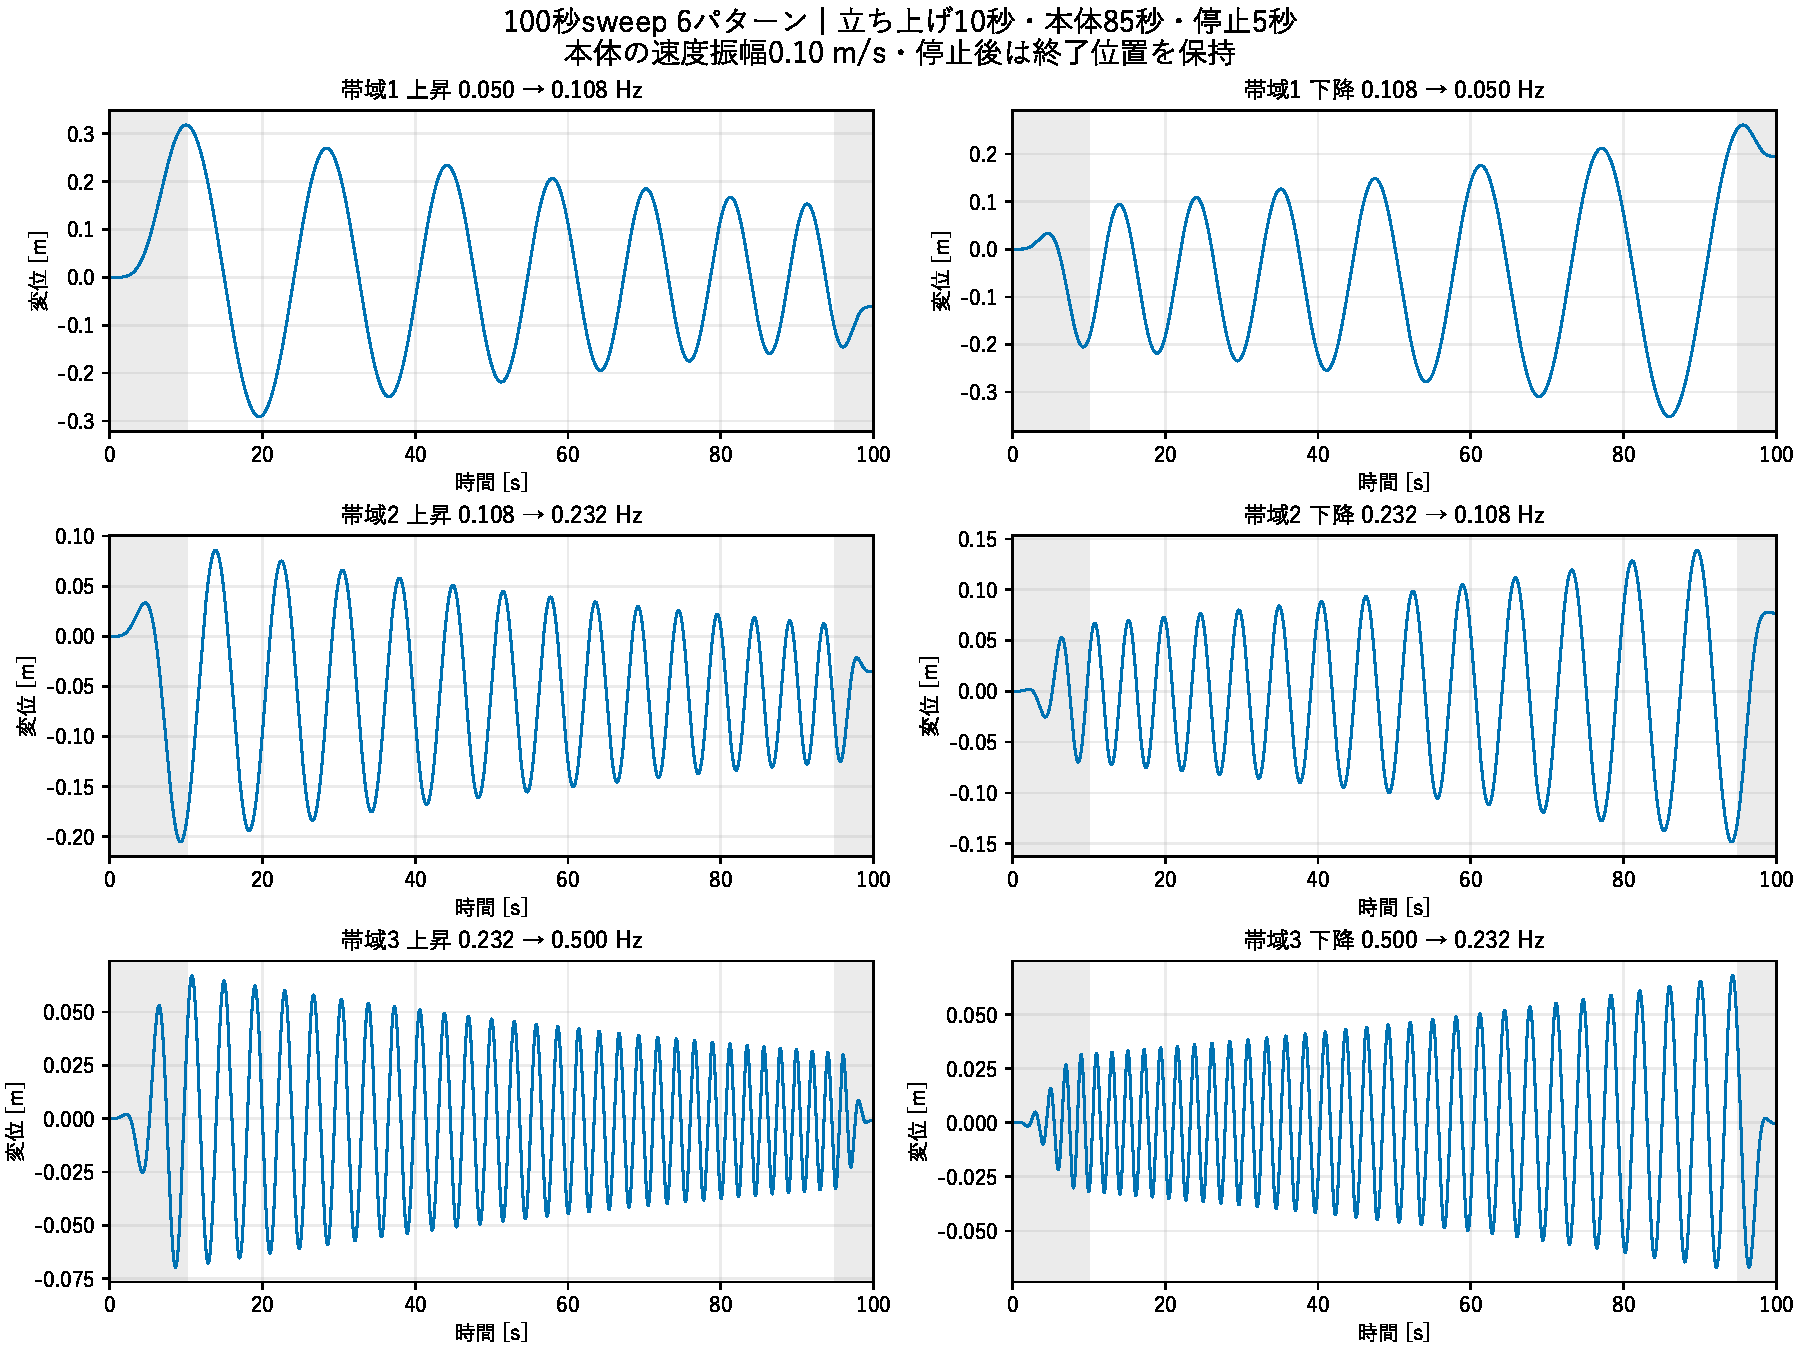
\includegraphics[width=\linewidth,height=116mm,keepaspectratio]{figures/sweep100_six_patterns.pdf}
\end{center}
\vspace{-6pt}
{\small\textbf{図2}\quad 6条件の変位波形。左が上昇、右が下降。灰色は立ち上げ・停止区間。
停止後は最終位置を保持し、原点復帰は行わない。各図の縦軸範囲は異なる。}

包絡に\(q(u)=10u^3-15u^4+6u^5\)を用い、
\begin{equation}
 e(t)=\begin{cases}
 q(t/10),&0\leq t<10,\\
 1,&10\leq t\leq95,\\
 q((100-t)/5),&95<t\leq100
 \end{cases}
\end{equation}
として、\(\dot\theta(t)=2\pi f(t)\)の位相を全区間で連続にする。
\begin{equation}
 v=0.10\,e\sin\theta,\qquad
 a=0.10\left(\dot e\sin\theta+e\,2\pi f\cos\theta\right),\qquad x=\int_0^t v(u)\,\mathrm du.
\end{equation}
位置は1 ms刻みで積分する。100秒で速度・加速度は0となり、その位置を保持する。
10秒の立ち上げは定常化の保証ではない。
波形と微分関係、端点、記録処理を自動テストで確認した。実機での追加提示は未実施。

{\footnotesize
選択肢は「100秒 分割sweep1--3」の上昇・下降。
定義元は\texttt{research\_sync/band\_sweeps.py}、描画は\texttt{waveform.js}。
\texttt{sweep100}に6条件のCSV・JSON・詳細図・最大値を保存。}
\end{document}
